\section{Online {\IterComp} Infrastructure} \label{sec:oic-infra}

Although {\itercomp} had been originally proposed as an \textit{offline} optimization strategy, it can also be adapted to work in online scenarios.
Instead of selecting the best optimization sequence as part of the development time (pre-shipping) of a program, a first version of the program is shipped together with an {\itercomp} mechanism.
In the online scenario, the program is shipped with an initial optimization sequence and different optimization sequences are evaluated as the end-user executes the program.
This optimization strategy is also known as idle-time optimization, as the re-compilation happens between runs of the program.

LLVM is particularly suitable for iterative compilation as it makes possible to cache a pre-compiled, but still unoptimized, version of the input program in the bitcode format of the LLVM IR.
This caching allows to speedup the time required for re-compilation as it is able to bypass the frontend phase.
If re-compilation time is critical, it would also be possible to keep only the hot portion of the code in the LLVM bitcode format, while the remaining portion of the code is already compiled to the final object code.
However, this is out of the scope of this paper and we always re-compile the whole program.

\begin{figure}[htb]
    \centering
    \includegraphics[width=\linewidth]{figs/infra-diagram}
    \caption{Overview of the execution engine for applying {\itercomp}.}
    \label{fig:infra-diagram}
\end{figure}
%\textbf{Describe the process step by step.}

Figure~\ref{fig:infra-diagram} shows an overview of the infrastructure required for applying online {\itercomp}
using WP as the metric of choice for evaluating optimization sequences.
The online {\itercomp} follows as described bellow:
\begin{enumerate}
\item The program is pre-compiled to the LLVM bitcode format without optimization.
\item The unoptimized program is instrumented for work profiling.
\item Execution-based optimization search:
 \begin{enumerate}
   \item The current optimization sequence is used for the re-compilation of the program.
   \item The program is executed with any input provided by the end-user.
         During the execution of the program, wall-clock time and the work metric are recorded by profiling instrumentation.
   \item If the recorded profiling for the current optimization can be used to compute an average performance measurement within a small confidence interval,
         then a new optimization sequence is generated.
         Otherwise, the same optimization sequence is used for the next execution.
 \end{enumerate}
\end{enumerate}

In this work, we focus mainly on the highlighted components.
The \textit{Work Instrumentation} phase focuses on providing a low-overhead instrumentation for profiling the work metric.
The instrumentation consists of adding a global counter to the program which is used to accumulate the amount of work computed during the program's execution, using the cost model of the instruction set.
A detailed description of the work instrumentation is presented in Section~\ref{chap:instr}.

Notice how the \textit{Work Instrumentation} phase is executed before performing any optimization to the program.
It is critical so that the work profiling always measure the same amount of work for a given input, regardless of the optimization sequence applied to the program.
Because the instrumentation is performed before optimising the program, it means that the work profiling derives the linear expression defined in Equation~\ref{eq:linear-work-expression}
based on the unoptimized program.
In other words, the basic blocks and the number of occurrences of the instruction in the basic blocks reflect the unoptimized program.
This particular sequence of compilation guarantees that the amount of work must is only input dependent, but consistent between different optimization sequences.

As the name suggests, the component called \textit{Optimization Selector} is responsible for selecting which optimization sequence to use for the next execution of the program.
It can either keep the same optimization sequence used in the previous execution or start monitoring the performance of a new optimization sequence.
An optimization sequence can be kept for multiple executions of the program in order to gather enough measurement to compute an average performance with small statistical deviations, i.e., for which the confidence interval has a small range.
We call by \textit{Input-Window Size} the number of executions performed using the same optimization sequence.

\subsection{Real Online Scenarios}

In most online scenarios, it is common for periods of peak usage and idle periods.
For example, mobile devices are usually intensely used during the day, with some idle periods usually when the battery is being re-charged~\citep{mpeis16}.
Similarly, many authors have also considered peak and idle (or underutilized) periods in the context of data centres~\citep{armbrust10,chen12b}.

The proposed infrastructure is very well suited for these real online scenarios\footnote{
However, if idle time is almost non-existent, the proposed infrastructure can still be used by re-compiling the program with a different optimization while multiple runs of the program are being executed.}.
In particular, periods of peak usage could be used to monitor multiple runs of the program using the same optimization sequence, collecting the work profiling and measuring its execution time,
while periods of idleness or underutilisation could be leveraged to use the profiling statistics for selecting better optimizations and re-compiling the program.
